\subsection{Motor}


El motor (Figura \ref{fig:motor}) asincrónico que se utiliza es de la marca \textbf{Altium} perteneciente a la firma \textbf{Schneider Electric}. Las especificaciones se muestran a continuación \\
\paragraph*{Altium Eff2}

\begin{minipage}[t]{.5\textwidth}
	\begin{itemize}
		\item Tipo: TE2A90SP2
		\item Tensión nominal: 380 V
		\item Corriente nominal: 3.46 A
		\item Frecuencia nominal:  50 Hz.
		\item Potencia: 1.5kW / 2 HP
		\item Fases: 3
		\item Factor de Potencia: 0.84
	\end{itemize}
\end{minipage}
\begin{minipage}[t]{.5\textwidth}
	\centering\raisebox{\dimexpr \topskip-\height}{%
		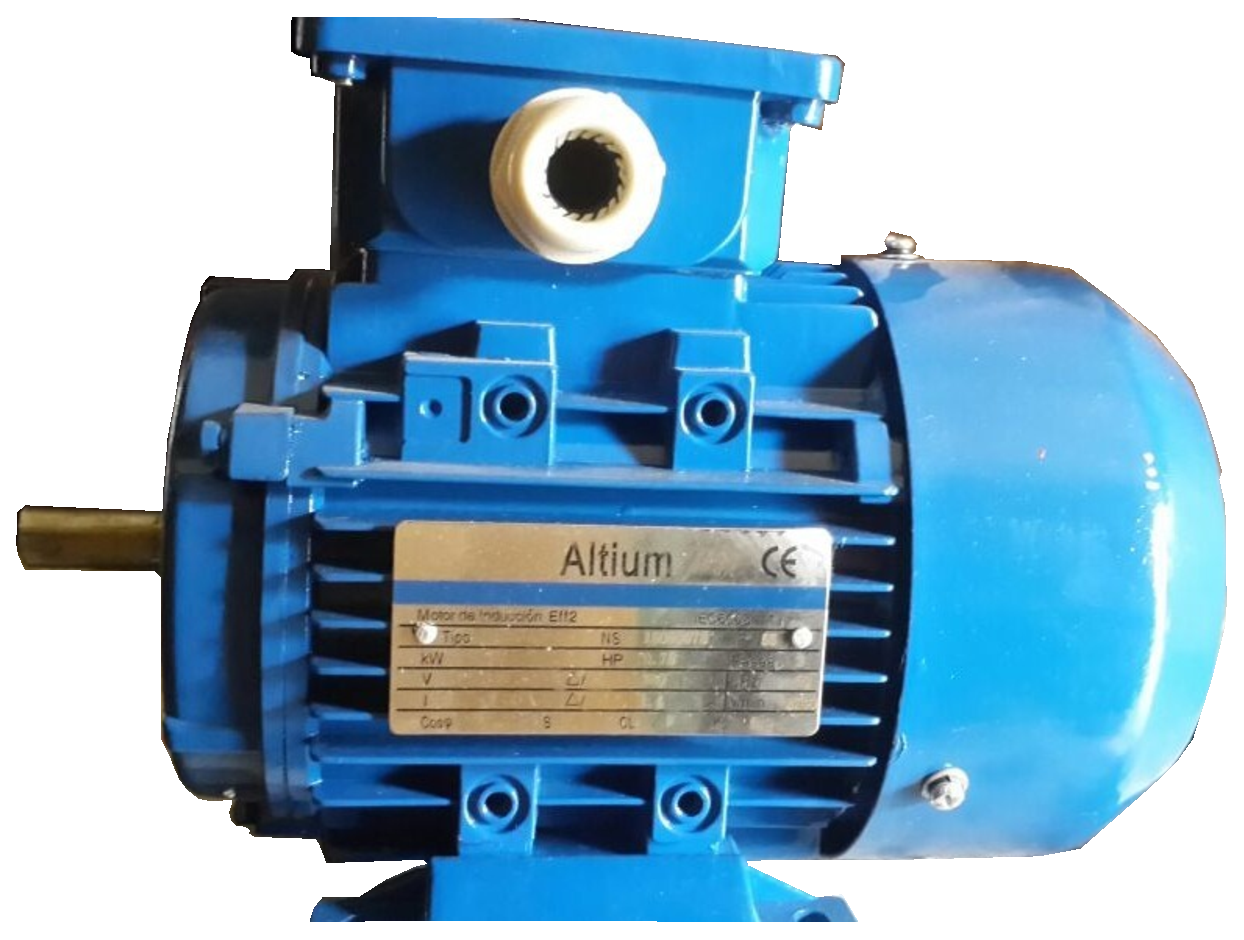
\includegraphics[scale=0.3]{motor.eps}}
	\captionof{figure}{Motor Altium}
	\label{fig:motor}

\end{minipage}

\subsection{Variador de velocidad}



El variador de velocidad que se utilizó pertenece a la marca \textbf{Schneider Electric} (Figura \ref{fig:variador}) y posee las siguientes características.
\paragraph*{Altivar 312}
\begin{minipage}[t]{.5\textwidth}
	\begin{itemize}
		\item 	Modelo: ATV312HU15N4
		\item   Tensión: 380-500 V
		\item 	Frecuencia: 50/60 Hz
		\item 	Potencia: 1.5kW / 2 HP
		\item 	Fases: 3
	\end{itemize}
\end{minipage}
\begin{minipage}[t]{.5\textwidth}
	\centering\raisebox{\dimexpr \topskip-\height}{%
		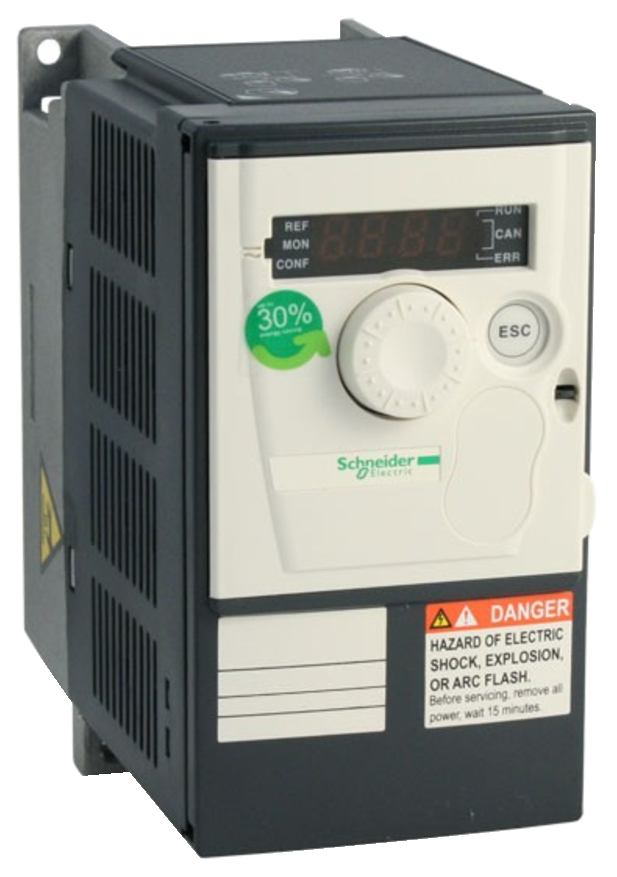
\includegraphics[scale=0.25]{variador.eps}}
	\captionof{figure}{Variador Altivar 312}
	\label{fig:variador}
\end{minipage}


%Cabe destacar que el variador estima la velocidad de acuerdo a los parámetros del motor, por lo que para medir la velocidad verdadera se utiliza un tacómetro perteneciente al laboratorio.


\subsection{Módulo didáctico PLC M340} \label{sec:didac}

El Laboratorio de Control de la UNPSJB cuenta con un módulo didáctico que posee un PLC modelo Modicom M340 de la empresa Schneider Electric. Esto cuenta con entradas analógicas, digitales, distintos métodos de comunicación y la capacidad de agregarle otros módulos según las necesidades de los proyectos a desarrollar en un riel.  \\
Los módulos con los que se cuenta son:
\begin{itemize}
	\item P342030
	\item DDM16022
	\item ART0414
	\item AMI0410 
	
\end{itemize}
%\url{http://instrumentacionycontrol.net/wp-content/uploads/2017/11/IyCnet_Hardware_Modicon_M340-min.pdf}
\begin{center}
	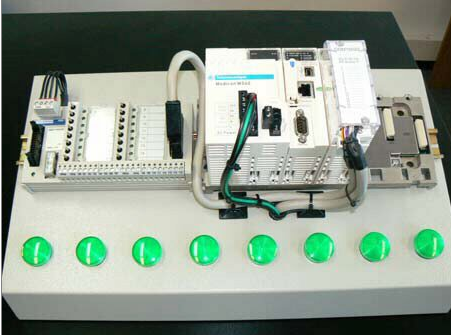
\includegraphics[width=0.7\linewidth]{educativo.png}
	\captionof{figure}{Módulo Didáctico PLC M340}
	\label{fig:didac}
\end{center}




